Ce chapitre concerne diff\'erents processus r\'eunis sous le terme cognition. Nous avons vu qu'il n'y a pas de distinction stricte entre la perception et la cognition puisque la derni\`ere influence la premi\`ere, mais nous nous int\'eresons ici aux aspects impliqu\'es dans la r\'esolution de probl\`emes. Nous nous int\'eressons aux fonctions que ces m\'emoires offrent \`a l'utilisateur d'un syst\`eme informatique.

La psychologie cognitive est une branche de la psychologie qui s'int\'eresse aux grandes fonctions de notre intellect. Nous nous int\'eresserons en particulier dans la m\'emoire, raisonnement, connaissances et apprentissage. D'autres aspects sont aussi important dans l'interaction personne-computer mais on va se concentrer sur les concepts fondamentaux. 

La psychologie cognitive porte un \textbf{regard fonctionnel} sur la m\'emoire. Elle d\'efinit trois types de m\'emoire qui correspondent \`a des fonctions cognitives distinctes:

\begin{itemize}
\item M\'emoire sensorielle: retient les \'even\'ements pass\'ess dans le dernier secondes.
\item M\'emoire de travail ou m\'emoire \`a court terme: retient les \'even\'ements pass\'ess dans les derniers dix minutes.
\item M\'emoire \`a long terme: retient les \'even\'ements pass\'ess \`a long terme. 
\end{itemize}

Le lien entre la fonction cognitive et le substrat biologique du cerveau est l'objet des \textbf{neurosciences}. Les trois m\'emoires d\'ecrites fonctionnellement (par performances ou oublis des sujets) ont \'et\'e mises en relation avec l'activation de zones distinctes du cerveau.Ces trois m\'emoires sont souvent pr\'esent\'ees comme des bo\^ites ou des tiroirs dans la grande armoire. C'est une simplification grossi\`ere. Une hypoth\`ese est par exemple que m\`emoire \`a court terme serait simplement un sous-ensemble de la m\'emoire \`a long terme qui a \'et\'e pr\'e-activ\'e. 

La mani\`ere la plus simple de comprendre notre cognition est d'analyser pourquoi nous commettons des erreurs.  On peut faire \c{c}a en mesurant la charge cognitive. Exemple: genealogy game. 

Normalement, la capacit\'e de notre m\'emoire de travail est limit\'ee entre cinq et neuf \'el\'ements. Pour la mesurer on peut utiliser:

\begin{itemize}
\item Mesures physiologiques: EEG, fr\'equence cardiaque, mouvement oculaires, contractions musculaires.
\item Mesures subjectives: par questionnaire apr\`es la t\^ache.
\item Mesures de performance: la "dual task".
\end{itemize}

La t\^ache 1 est de difficult\'e constante alors qu'on augmente progressivement la difficult\'e de la t\^ache 2. \`A un certain seuil de difficult\'e, la difficult\'e de la t\^ache 2 va conduire \`a une augmentation du nombre d'erreurs sur la t\^ache 1, bien que celle-ci n'ait pas augment\'e en difficult\'e. Cette interf\'erence d'une t\^ache sur l'autre t\'emoigne d'une surcharge cognitive.

\begin{figure}[H]
\centering
\makebox[\textwidth][c]{
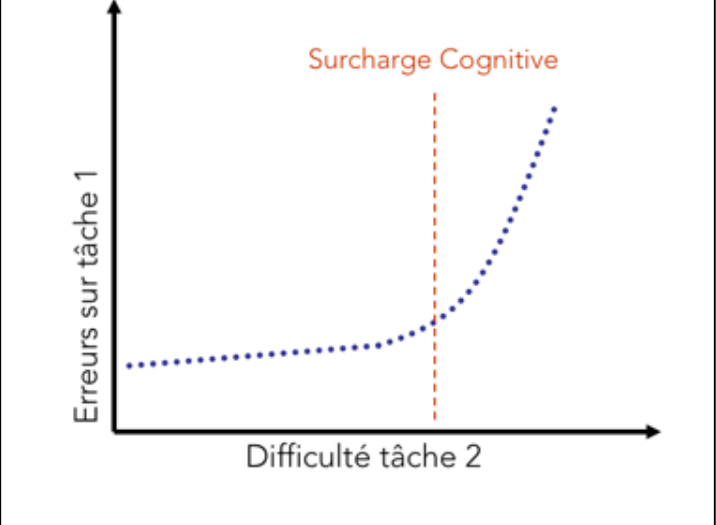
\includegraphics[scale=0.35]{./images/dual.png}
}
\end{figure}

Est-il vraiment possible que nous puissions r\'esoudre des t\^aches complexes, telles que la programmation, avec une m\'emoire de travail qui serait limit\'ee \`a sept slots? Lorsqu'on programme, on est totalement concentr\'e afin de maintenir en m\'emoire le nom des variables, des fonctions ou des classes utilis\'ees, leur position dans le code, les sous-fen\^etres, etc. 

\begin{figure}[H]
\centering
\makebox[\textwidth][c]{
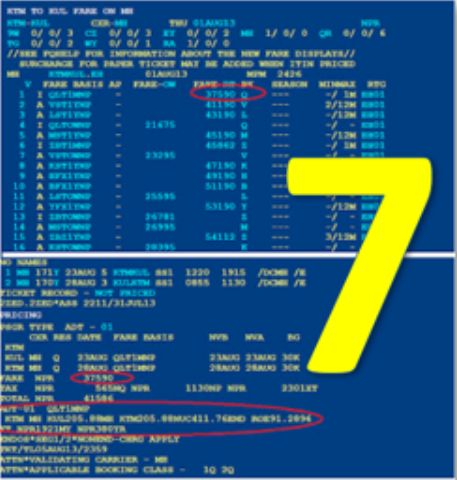
\includegraphics[scale=0.35]{./images/prof.png}
}
\end{figure}

Ce type d'interface est utilis\'ee par les professionnels pour r\'eserver des billets d'avion. \`A la diff\'erence de l'interface web que nous utilisons pour r\'eserver un vol cette interface contient une quantit\'e \'enorme d'information. Comment les utilisateurs peuvent-ils g\'erer cette quantit\'e alors qu'ils ont les m\^emes limites que tout le monde en termes de charge cognitive? Un utilisateur expert lit en fait cet \'ecran non comme 545 \'el\'elements mais comme un nombre limit\'e de blocs d'information.

De la m\^eme mani\`ere un conducteur expert parvient \`a mener un grand nombre d'op\'erations en parall\`ele. Lorsqu'on apprend \`a conduire, changer de vitesse repr\'esente plusieurs op\'erations cognitives distinctes. Plus tard, ce jeu d'op\'erations ayant \'et\'e automatis\'e ou "compil\'e", il ne mobilise plus qu'une partie mineur de notre m\'emoire de travail. Les interfaces proposent aussi des moyes de compilation. Il existe de nombreuses \'etudes qui diff\'erencient novices et experts. La compilation des connaissances est l'un des \'el\'ements, mais ce n'est pas le seul.

\subsection{Split attention effect}

L'effet de "split attention" d\'ecrit l'augmentation de la charge cognitive qu'implique les aller-retours visuels entre une figure et sa l\'egende, ou, de mani\`ere plus g\'en\'erale, entre deux sources d'information. Combien d'informations par \'ecran est-il optimal de pr\'esenter dans un seul \'ecran? Minimiser les information par \'ecran n'est pas la solution car la plupart des t\^aches demandent de mettre en relation plusieurs \'el\'ements d'information. D\'ecomposer l'information en n \'ecrans n'est pas id\'eal puisque cela aboutit \`a la morceler. Le fait de structurer l'information r\'eduit la charge cognitive. 

\begin{figure}[H]
\centering
\makebox[\textwidth][c]{
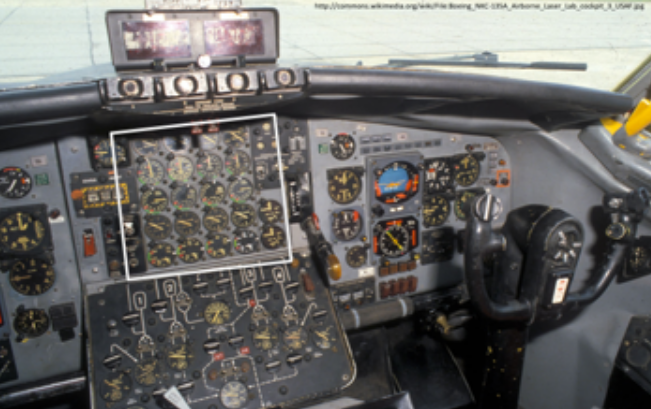
\includegraphics[scale=0.35]{./images/structure.png}
}
\end{figure}

Par exemple, si n cadrans ont des aiguilles qui devraient \^etre parall\`eles, le contr\^ole de ces n \'ecrans ne n\'ecessite pas de lire les indications de chaque cadran car il suffit de contr\^oles le parall\'elisme.


On peut calculer la charge cognitive avec la fomule suivante:

$$\text{Charge cognitive} = \frac{\text{Quantit\'e d'information}}{\text{Niveau d'expertise} \cdot \text{Qualit\'e du design}}$$

Ici le design de l'interface est la seule variable sur laquelle nous avons de l'influence. 

\subsection{Distributed cognition}

Distributed cognition is an approach to cognitive science research that deploys models of the extended mind by taking as the fundamental unit of analysis "a collection of individuals and artefacts and their relations to each other in a particular work practice".

Par exemple un programmeur utilise l'\'ecran pour \'etendre sa m\'emoire de travail car elle pr\'esent l'ensemble des informations n\'ecessaires \`a r\'ealiser son travail. Une personne aveugle utilise sa canne pour explorer l'espace. L'id\'ee c'est d'\'etudier le syst\`eme cognitif dans son ensemble, compos\'e d'un ou plusieurs cerveaux et de leurs outils.

Dans la m\'emoire \`a long terme, on distingue deux formes de connaissances: connaissances d\'eclaratives et connaissances proc\'edurales. Les connaissances d\'eclaratives comprennent les concepts, id\'ees, principes, faits ou th\'eories. Les connaissances proc\'edurales d\'ecrivent les mani\`eres d'op\'erer, faire, d\'ecomposer ou calculer. Il y a une r\'ealimentation entre les deux. 

Dans l'ensemble des connaissances d\'eclaratives on distingue la m\'emoire s\'emantique et la m\'emoire \'episodique. La m\'emoire s\'emantique retient les faits, concepts ou d\'efinitions. La m\'emoire \'episodique retient les ev\'enements pass\'es ou imagin\'es. 

\begin{figure}[H]
\centering
\makebox[\textwidth][c]{
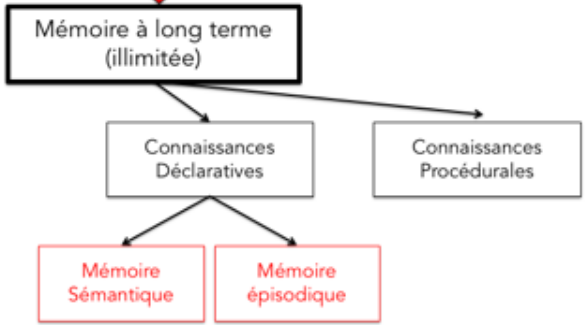
\includegraphics[scale=0.35]{./images/semantique.png}
}
\end{figure}

A \textbf{mental model} is an explanation of someone's thought process about how something works in the real world.

La m\'emoire s\'emantique aide \`a construire les mod\`eles mentaux. Ce mod\`eles evoluent avec l'exp\'erience et sont souvent li\'es au contexte dans lequel ils ont \'et\'e acquis. Ils ne sont pas forc\'ement corrects, ni complets et ils peuvent comprendre des contradictions. Il s'agit des explications simplifi\'ees des ph\'enom\`enes complexes et contiennent une estimation de leur validit\'e qui permet de les utiliser malgr\'e leur incertitude. Ils aident \`a comprendre certaines erreurs des utilisateurs.

\subsection{Metacognition}

La metacognition d\'esigne la connaissance des connaissances ("je ne suis pas bon pour m\'emoriser les noms", "je suis pr\^et pour l'examen", "pour des probl\`emes de ce type, je pr\'ef\`ere faire un sch\'ema") et le raisonnement sur le raisonment ("je devrais repartir d'un \'etape pr\'ec\'edente" ou quelle est la meilleure m\'ethode pour ce probl\`eme?).

\begin{figure}[H]
\centering
\makebox[\textwidth][c]{
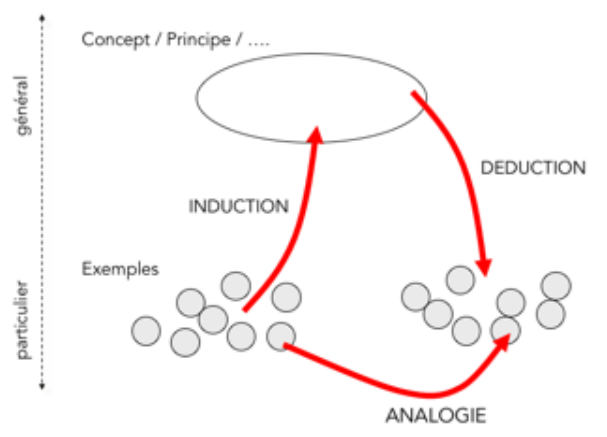
\includegraphics[scale=0.35]{./images/principes.png}
}
\end{figure}


\subsection{Exercises}

\begin{figure}[H]
\centering
\makebox[\textwidth][c]{
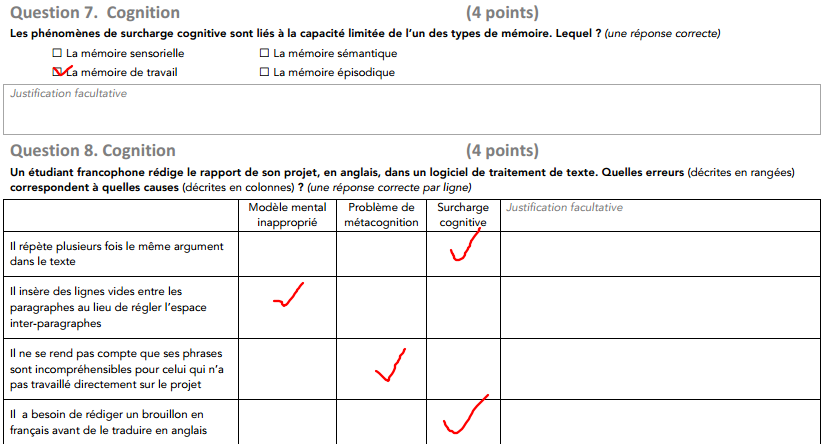
\includegraphics[scale=0.55]{./images/exercise3.png}
}
\end{figure}
























